\chapter{Rupture framework}\label{rupture}

In this chapter, we will describe our framework for conducting compression side-channel attacks,
Rupture. Rupture is a service-based architecture system which contains multiple
independent components.

The section \ref{sec:assumptions} descibes in details the assumptions needed to be made 
in order to orchestrate the attack. The section \ref{sec:principles} describes the 
terminology used in our framework and its governing principles. Finally, the section
\ref{sec:architecture} presents thoroughly the multiple components.
While the components are designed to be able to run
independently on different networks or computer systems, easy instances of the
attack can be performed by running all subsystems on an individual system. We
provide appropriate scripts to conduct such attacks easily.


\section{Attack Assupmtions}\label{sec:assumptions}

The attack framework assumes a \textit{target} service to be attacked. Typically
this target service is a web service which uses TLS. Specifically, we are
targeting services that provide HTTPS end-points. However, this assumption can
be relaxed and attacks against other similar protocols are possible. Any
protocol that exchanges encrypted data on the network and for which a
theoretical attack exists can in principle be attacked using Rupture. We
designed Rupture to be a good playground for experimentation for such new
attacks. Examples of other encrypted protocols for which attacks can be tested
include SMTP and XMPP.

The attack also assumes a user of the target service for which data will be
decrypted, the \textit{victim}. The victim is associated with a particular target.

There are two underlying assumptions in our attack: The injection and the
sniffing assumptions. These are often achieved through the same means, although
not necessarily.

The injection assumption states that the adversary is able to
inject code to the victim's machine for execution. This code is able to issue
adaptive requests to the target service. Injection in Rupture is achieved
through the \textit{injector} component. The code that is injected is the \textit{client}
component.

The sniffing assumption states that the adversary is able to observe network
traffic between the victim and the target. This traffic is typically
ciphertexts. Sniffing is achieved through the \textit{sniffer} component.

Both the referenced \textit{sniffer} and \textit{client} will be presented in section 
\ref{sec:architecture}.



\section{Principles of Attack}\label{sec:principles}


The attack takes place by first injecting client code into the victim's
computer using the injector. The client then opens a command-and-control
channel to the real-time service, which forwards work from the backend to the
client.

When a client associated with a victim asks to work, the backend passes a work
request to the real-time service, which passes it to the client. These work
requests ask the client to perform a series of network requests from the
victim's computer to the target web app. As these requests are made from the
victim's browser, they contain authentication cookies which authenticate the
user to the target service. As such, the responses contain sensitive data, but
that data is not readable by the client due to same-origin policy.

When a response arrives from the target web app to the victim's computer, the
encrypted response is collected by the sniffer on the network. The encrypted
data pertaining to one response is a \textit{sample}. Each work request asks for
multiple requests to be made, and therefore multiple samples are collected per
work request. The set of samples collected for a particular work request are a
\textit{sampleset}.

A successful attack completely decrypts a portion of the plaintext. The portion
of the plaintext which the attack tries to decrypt is the \textit{secret}. That
portion is identified through an initially known prefix which distinguishes it
from other secrets. This prefix is typically 3 to 5 bytes long. Each byte of
the secret can be drawn from a given \textit{alphabet}, the secret's alphabet. For
example, some secrets only contain numbers, and so their alphabet is the set of
numbers [0-9].

At each stage of the attack, a prefix of the secret is known, because that
portion of the secret has already been successfully decrypted. The prefix
decrypted grows until the whole secret becomes known, at which stage the attack
is completed.

When a certain prefix of the secret is known, the next byte of the secret must
be determined. The attack initially assumes the next unknown byte of the secret
can come from the secret's alphabet, but slowly drills down and rejects
alphabet symbols until only one candidate symbol remains. At each stage of the
attack of one byte of the secret, there is a certain **known alphabet** which
the next byte can take. This known alphabet is a subset of the secret's
alphabet.

To drill down on the known alphabet, one of two methods is employed. In the
\textit{serial method}, each symbol of the known alphabet is tried sequentially. In
the \textit{divide \& conquer method}, the alphabet is split into two \textit{candidate
alphabet} subsets which are tried independently.

The attack is conducted in \textit{rounds}. In each round, a decision is made
about the state of the attack and more becomes known about the secret. In a
round, either the next byte of the secret becomes known, or the known alphabet
is drilled down to a smaller set. In order to compare various different
candidate alphabets, the attack executes a series of \textit{batches} of data
collection for each round.

In each batch, several samples are collected from each probability distribution
pertaining to a candidate alphabet, forming a sampleset. When samplesets of the
same amount of samples each have been collected for all the candidate
alphabets, a batch is completed and the data is analyzed. The analysis is
performed by the **analyzer** which statistically compares the samples of
different distributions and decides which distribution is optimal, i.e.
contains the correct guess. This decision is made with some \textit{confidence},
which is expressed in bytes. If the confidence is insufficient, an additional
batch of samplesets is collected, and the analysis is redone until the
confidence value surpases a given threshold.

Once enough batches have been collected for a decision to be made with good
confidence, the round of the attack is completed and more information about the
secret becomes known. Each round at best collects one bit of information of the
secret.

\section{Architecture}\label{sec:architecture}


\subsection{Injector}
The injector component is responsible for injecting code to the victim's
computer for execution. In our implementation, we assume the adversary controls
some network of the victim. Our injector injects the client code in all
unauthenticated HTTP responses that the victim receives. This Javascript code
is then executed by the victim's browser in the context of the respective
domain name. We use bettercap \cite{bettercap}  to perform the HTTP
injection. The injection is performed by ARP spoofing the local network and
forwarding all traffic in a Man-in-the-Middle manner. It is simply a series of
shell scripts that use the appropriate bettercap modules to perform the attack.

As all HTTP responses are infected, this provides increased robustness.
The injected client code remains dormant until it is asked to wake
up by the command-and-control channel. This means that the user can switch
between browsers, reboot their computer, close and reopen browser tabs, and the
attack will keep running.

The injector component needs to run on the victim's network and as such is
light-weight and stateless. It can be easily deployed on a machine such as a
Raspberry Pi, and can be used for massive attacks, for example at public
unencrypted networks such as coffee shops or airports. Multiple injectors can
be deployed to different networks, all controlled by the same central
command-and-control channel.

While injection is performed on the local network through altering HTTP
responses in our case, the injector component is independent and can be
replaced by alternative means. Other good points of injection that can be used
instead of our build-in injector are giving a link directly to the victim via a
phishing mail, in which case attack robustness is limited, or by injecting code
at the ISP or router level if the adversary has such a level of access.


\begin{figure}[H] \caption{Injector Code} \centering
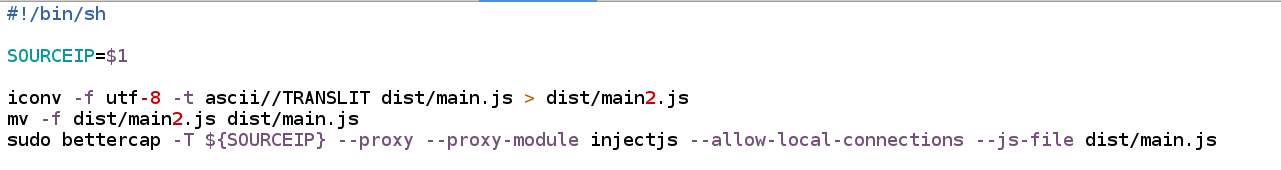
\includegraphics[width=0.7\textwidth]{diagrams/injector.png}\end{figure}


\subsection{Sniffer}

The sniffer component is responsible for collecting data directly from the
victim's network. As the client issues chosen plaintext requests, the sniffer
collects the respective ciphertext requests and ciphertext responses as they
travel on the network. These encrypted data are then transmitted to the backend
for further analysis and decryption.

Our sniffer implementation runs on the same network as the victim. It is a
Python program which uses scapy \cite{scapy} to
collect network data.

Our sniffer runs on the same machine as our injector and utilizes the
injector's ARP spoofing to retrieve the data from the wire or the air. 
Other sniffer alternatives include sniffing data on the target network side, or
on the ISP or router point if the adversary has such a level of access.

The sniffer exposes an HTTP API which is utilized by the backend for
controlling when sniffing starts, when it is completed, and to retrieve the
data that was sniffed. This API is described below.


\subsubsection{backend <-> sniffer (HTTP)}

The Python backend application communicates with the sniffer server, in order
to initiate a new sniffer, get information or delete an existing one. The  sniffer 
server implements a RESTful API for communication with the backend.

\textbf{/start} is a POST request that initializes a new sniffer.
Upon receiving this request, the sniffer service should start sniffing.

The request contains a JSON with the \textit{source\_ip}, 
- the IP of the victim on the local network - and the \textit{destination\_host}
- the hostname of the target that is being attacked.

The backend returns \textit{HTTP 201} if the sniffer is created correctly. Otherwise, it returns
\textit{HTTP 400} if either of the parameters is not properly set, or \textit{HTTP 409 -
Conflict}, if a sniffer for the given arguments already exists.

\textbf{/read} is GET request that asks for the network capture of the sniffer.

The GET parameters are the \textit{source\_ip}  - the IP of the victim on the local network -
and the \textit{destination\_host} - the hostname of the target that is being attacked.

The backend returns \textit{HTTP 200} with a JSON that has a field \textit{capture}, which contains the
network capture of the sniffer as hexadecimal digits, and a field \textit{records},
that contains the total amount of captured TLS application records. In case of
error, \textit{HTTP 422 - Unprocessable Entity} is returned if the captured TLS
records were not properly formed on the sniffed network, or \textit{HTTP 404} if no
sniffer with the given parameters exists.

\textbf{/delete} is a POST request that asks for the deletion of the sniffer

The request contains a JSON with the \textit{source\_ip} - the IP of the victim on the local network - 
and \textit{destination\_host} - the hostname of the target that is being attacked.

The backend Returns \textit{HTTP 200} if the sniffer was deleted successfully, or \textit{HTTP 404} if 
there is no sniffer with the given parameters.

\subsection{Client}

The client runs on the victim machine and is responsible for issuing adaptive
chosen plaintext requests to the target oracle.

The client is written in Javascript and runs in a different context from the
target website. Thus, it is subject to same-origin policy and cannot read the
plaintext or encrypted responses. However, the encrypted requests and responses
are available to the sniffer through direct network access.

The client contains minimal logic. It connects to the real-time service through
a command-and-control channel and registers itself there. Afterwards, it waits
for work instructions by the command-and-control channel, which it executes.
The client does not take any decisions or receive data about the progress of
the attack other than the work it is requested to do. This is intentional so as
to conceal the workings of the adversary analysis mechanisms from the victim in
case the victim attempts to reverse engineer what the adversary is doing.
Furthermore, it allows the system to be upgraded without having to deploy a new
client at the victim's network, which can be a difficult process.

As a regular user is browsing the Internet, multiple clients will be injected
in insecure pages and they will run under various contexts. All of them will
register and maintain an open connection through a command-and-control channel
with the real-time service. The real-time service will enable one of them for
this victim, while keeping the others dormant. The one enabled will then
receive work instructions to perform the required requests. If the enabled
client dies for whatever reason, such as a closed tab, one of the rest of the
clients will be waken up to take over the attack.

The client is a Javascript program written using harmony / ECMAScript 6 and
compiled using babel and webpack.


\subsection{Real-time}

The real-time service is a service which awaits for work requests by clients.
It can handle multiple targets and victims. It receives command-and-control
connections from various clients which can live on different networks,
orchestrates them, and tells them which ones will remain dormant and which ones
will receive work, enabling one client per victim.

The real-time service is developed in Node.js.

The real-time service maintains open web socket command-and-control connections
with clients and connects to the backend service, facilitating the
communication between the two.

The real-time server forwards work requests and responses between the client
and the Django service. The communication it does with the client uses web
sockets in order to achieve bi-directional communication in real-time. This
also facilitates the ability to detect that a client has gone away, which is
registered as a failure to do work. This can happen for example due to network
errors if the victim disconnects from the network, closes their tab or browser,
and so on. It is imperative that incomplete work is marked as failed as soon as
possible so that the attack can continue by recollecting the failed samples.

The web socket API exposed by the real-time service is explained below.

\subsubsection{client <-> real-time protocol}

The client / real-time protocol is implemented using socket.io websockets.

 \textbf{client-hello / server-hello}

When the client initially connects to the real-time server, it sends the message
\textit{client-hello} passing its \textit{victim\_id} to the real-time server.  The server
responds with a \textit{server-hello} message. After these handshake messages are
exchanged, the client and server can exchange futher messages.

 \textbf{get-work / do-work}

When the client is ready to perform work, it emits the message **get-work**
requesting work to be performed from the real-time server. The real-time server
responds with a **do-work** message, passing a *work* object, that is
structured as defined below:

\texttt{
typedef work \\
  amount: int \\
  url: string \\
  timeout: int (ms) \\
}

If the real-time service is unable to retrieve work from the backend due to a
communication error, real-time will return an empty work object indicating
there is no available work to be performed at this time.

 \textbf{work-completed}

When the client has finished its work or has been interrupted due to network
error, it emits a \textit{work-completed} message, containing the following
information:

\texttt
{
  work: work,
  success: bool
}


\textit{success} is \textit{true} if all requests were performed correctly, otherwise it
is \textit{false}. \textit{work} contains the work that was performed or failed to perform.

\subsection{Backend}

The backend is responsible for strategic decision taking, statistical analysis
of samples collected, adaptively advancing the attack, and storing persistent
data about the attacks in progress for future analysis.

The backend talks to the real-time service for pushing work out to clients. It
also speaks to the sniffer for data collection.

It is implemented in Python using the Django framework.

The backend exposes a RESTful API via HTTP to which the real-time service
makes requests for work. This API is explained below.

\subsubsection{real-time -> backend (HTTP)}

The backend implements various API endpoints for communication with the
real-time server.


\textbf{/get\_work/<victim>} is an HTTP GET endpoint. It requests work to 
be performed on behalf of a client. The argument passed is the \textit{victim}
- the id of the victim.

If there is work to be done, it returns an \textit{HTTP 200} response with the JSON
body containing the work structure. The work will contain instructions to
collect multiple samples from the same distribution by performing a series of
similar requests. The samples associated with a particular work request and
performed all together constitute a \textit{sampleset}.

In case no work is available for the client, it returns an HTTP `404` response.
Work can be unavailable in case a different client is already collecting data
for the particular victim, and we do not wish to interfere with it.

\textbf{/work\_completed/<victim>} is an HTTP POST endpoint. It indicates on behalf 
of the client that some work was successfully or unsuccessfully completed. The arguments
passed are the \textit{work} and a boolean \textit{success} parameter

If \textit{success} is \textit{True}, this indicates that the series of indicated requests
were performed by the victim correctly. Otherwise, the victim failed to perform
the required requests due to a network error or a timeout and the work has to
be redone.


